\documentclass[11pt]{article}
\usepackage{tocloft}
\usepackage{graphicx}
\usepackage{calc}
\usepackage{amssymb}
\usepackage{color}
\usepackage{array}
\usepackage[sc]{mathpazo}
\usepackage{url}
\usepackage[final]{pdfpages}

%\linespread{1.05}
\oddsidemargin=0pt
\evensidemargin=0pt
\textwidth=6.5in
\topmargin=0pt
\headheight=0pt
\headsep=0pt
\textheight=9in
% EXPERIMENTAL
%\parindent=0pt
%\parskip=3pt
\setlength{\parindent}{0cm}
\newcommand\secfont{\fontfamily{cmss}\selectfont}%\textwidth 5.5truein
\newcommand\pifheading[1]{{\secfont\textbf{#1}:}}
%\oddsidemargin -0.40truein
%\textheight 8.0truein
%\topmargin -0.25truein
\def\lo{
\mathrel{\raise.3ex\hbox{$<$}\mkern-14mu\lower0.6ex\hbox{$\sim$}}
}
\def\hi{
\mathrel{\raise.3ex\hbox{$>$}\mkern-14mu\lower0.6ex\hbox{$\sim$}}
}

\textwidth = 6.6 in
\textheight = 9.1 in
\oddsidemargin = -0.05 in
\evensidemargin = +0.05 in
\topmargin = -.1 in
\headheight = 0.0 in
\headsep = 0.0 in
\parskip = 0.06in
\newcommand\registered{{\ooalign{\hfil\raise .00ex\hbox{\scriptsize R}\hfil\crcr\mathhexbox20D}}}

%% Define a new 'leo' style for the package that will use a smaller font.
\makeatletter
\def\url@leostyle{%
  \@ifundefined{selectfont}{\def\UrlFont{\sf}}{\def\UrlFont{\small\ttfamily}}}
\makeatother
%% Now actually use the newly defined style.
\urlstyle{leostyle}

%\pagestyle{empty}
%\includeonly{previous,proposal_references}
%\includeonly{proposal_references}
%\includeonly{previous}

% TOC

\begin{document}
%%%%%%%%%%%%%%%%%%%%%%%%%%%%%%%%%%%%%%%%%%%%%%%%%%%%%%%%%%%%%%%%%%%%%

% By Scott Bassler
% Modifications by Walter Freeman

\begin{center}
\textbf{\Large
AST101: Our Corner of the Universe \\
\vspace*{0.1cm}
Lab 1: Stellarium and the Celestial Sphere
}
\end{center}

\vspace*{0.5cm}

\hrule
{\Large Name:}\vspace*{0.5cm}\\\hrule
{\Large Student number (SUID):}\vspace*{0.5cm}\\\hrule
{\Large Lab section:}\vspace*{0.5cm}\\\hrule
{\Large Group Members:}\vspace*{0.5cm}\\\hrule
\vspace*{0.5cm}

%%%%%%%%%%%%%%%%%%%%%%%%%%%%%%%%%%%%%%%%%%%%%%%%%%%%%%%%%%%%%%%%%%%%%
\section{Introduction}

Having done the prelab, you should be acquainted with the basics of how to use Stellarium. Now, we'll use it to take a good look at the basic motions of the sky, and see how the Celestial Sphere model developed. We'll also take an early look at the motion of perhaps the most important object in the entire sky: the Sun!

\subsection*{Materials}

This lab makes extensive use of Stellarium. If you do not have your own computer with Stellarium installed, you may borrow one of the laptops in the classroom from your TA. Do not take this laptop with you! Remember, you're supposed to be working in groups, and not everyone needs to have one.

\subsection*{Objective}

To see with your own eyes the motions of the sky described during the lecture, and to get a better understanding of the concepts described.

\newpage

\section{First Look at the Celestial Sphere}

\subsection{Can You Tell What's Spinning?}

Today, we take it for granted that the Earth moves around the Sun, and that the Earth spins on its axis, creating the apparent motion of the night sky. In short, the Earth does most of the moving. But that wasn't obvious to ancient astronomers. The early Greeks thought that the sky was this grand Celestial Sphere that spun around the Earth, and the objects on the sky were bound to it. The apparent motion of the celestial objects was due mostly to the sphere spinning, as well as the ability for some objects like the Sun to move along the sphere.

\noindent
\textbf{Question 1.} Before you turn on your computer, let's see how such a mistake could be made. Stand up, and have your group mates stand around you. Get out a smartphone, and record a video while you slowly spin in place. 

Then, stop spinning, but have everyone in your group move in a circle around you while you record another video.\\

If you pay attention only to your group mates and not the background behind them, could you easily tell whether you were spinning, or whether they were spinning around you, from looking at the two videos?\\
\vspace*{1.5cm}

\hrulefill\\
\noindent

\textbf{Question 2.} Now, boot up Stellarium. Don't worry about the time or location, but turn off the atmosphere so you can 
see the stars even during the daytime.
(There is a button along the bottom menu, or use the hotkey A). Now, increase the time speed so that you can actually see the stars move. Looking at the sky, can you tell whether the planet in Stellarium is spinning, or whether the sky is moving around it?\\
\vspace*{1.5cm}


\hrulefill\\

\newpage

\section{Motion Of The Stars}

\subsection{Star Paths Of Syracuse}

\textbf{Question 3.} Leaving the atmosphere off, set your location to Syracuse. Point your camera to the east. Are the stars rising or setting in the east? If you can't see them moving, change the rate at which time passes so you can see stars moving slowly in
the sky.

\vspace*{1.5cm}

\hrulefill\\
Stand up, and trace the paths of the stars in the actual sky with your finger as they move past on the Stellarium display. (You'll need to figure out which way is East.) \\


\textbf{Question 4.} Now, point your camera to the west. Are the stars rising or setting? Again, trace the paths that the stars follow
with your finger in the actual sky.\\
\vspace*{1.5cm}

\hrulefill\\   

\textbf{Question 5.} After rising, do the stars go to the northern sky, or the southern sky?\\
\vspace*{1.5cm}

\hrulefill\\

\textbf{Question 6.} Some stars never rise or set, but instead stay above the horizon the entire day. Such stars are called \textbf{circumpolar} stars. Are there any circumpolar stars in Syracuse? What part of the sky are they in?\\
\vspace*{1.5cm}

\hrulefill\\
\newpage
\textbf{Question 7.} What is at the center of the motion of the circumpolar stars? Does this point have a special name?\\
\vspace*{1.5cm}

\hrulefill\\

\textbf{Question 8.} Point Stellarium's view back to the north, and line your computer up so that the view matches the real world --
so that, when you look at your computer screen, you are looking north. Click on one star to highlight it. Then, all three people
in your group should point at the location in the {\it actual} sky where you could find that star. 

Then, set the rate at which time passes so you can see the stars moving slowly. As the star moves on the computer screen, follow
its path in the {\it actual} sky with your fingers.

(All three people in your group should share one computer for this)

Then, set your view in Stellarium to the east. Mark a star as it rises over the eastern horizon; do the same thing. Your group
should follow the path of this star as it moves through the sky, rising and setting and rising again.

\textbf{Question 9.} Have your TA make sure you've done this correctly and sign your lab below before moving on!\\ \\

\hrulefill

\textbf{Question 10.}Where is the star you marked in the previous question after it has set? Why can't you see it then?
\vspace*{1.5cm}

\hrulefill\\

\newpage

\textbf{Question 11.} On the diagram below, sketch the paths of the stars viewed from Syracuse. Make sure to include circumpolar stars, and label the North Celestial Pole (NCP). \\
\vspace*{1.5cm}

%\begin{center}
%	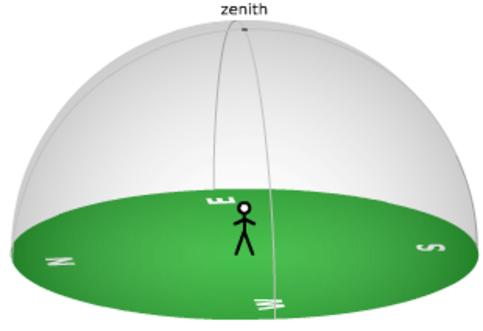
\includegraphics{local_sky}
%\end{center}

\subsection{Stars At The Equator And North Pole}

\textbf{Question 12.} Set your location to the equator (You can either find a location at the equator, or just set the latitude to 0). At the equator, where do the stars rise? Where do they set? \\
\vspace*{1.5cm}

\hrulefill\\

\textbf{Question 13.} At the equator, is the NCP visible? What about the SCP (South Celestial Pole)? Where can they be found? \\
\vspace*{1.5cm}

\hrulefill\\

\newpage

\textbf{Question 14.} Sketch the paths of the stars for the equator below. Be sure to include the NCP and SCP if they are visible. \\
\vspace*{1.5cm}

\begin{center}
	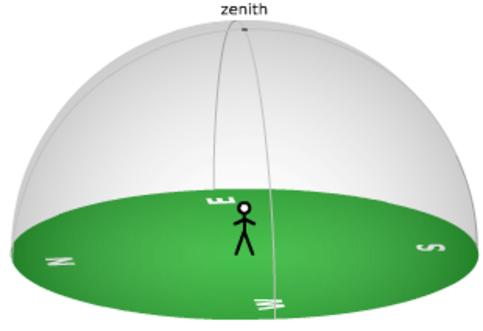
\includegraphics{local_sky} 
\end{center}

\textbf{Question 15.} Set your location to the North Pole (latitude of $90^\circ$). Where do the stars rise and set here? Can you see the NCP or SCP?\\
\vspace*{1.5cm}

\hrulefill\\

\textbf{Question 16.} Sketch the paths of the stars for the north pole below. Be sure to include the NCP and SCP if they are visible. \\
\vspace*{1.5cm}

\begin{center}
	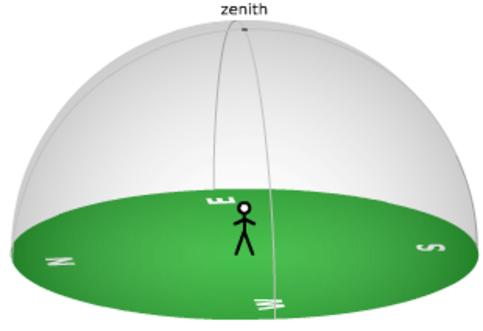
\includegraphics{local_sky}
\end{center}

\newpage

\section{Motion Of The Sun}

\subsection{Peak Of The Sun}

\textbf{Question 17.} Make sure your location is set to Syracuse New York, and set the time to be 6am on September 21, 2019. Advance time (remember you can speed up time!) until the Sun is at its highest point in the sky; that is, it's at its the highest it ever gets above the ground. When the Sun is at its highest point, where is it (North, South East, etc.)?\\
\vspace*{1.5cm}

\hrulefill\\

\textbf{Question 18.} Do the same for March 21. Where is the Sun highest in the sky?\\
\vspace*{1.5cm}

\hrulefill\\

\textbf{Question 19.} With the Sun at its highest point in the sky. advance time forward by 1 solar day (Hotkey =) many times. Does the Sun's height in the sky stay the same?\\
\vspace*{1.5cm}

\hrulefill\\

\textbf{Question 20.} Continue adding solar days until the Sun is at its highest point during the year. Around what date does this occur? What is the date for when the Sun is at its lowest point? Are these days special in some other way?\\
\vspace*{1.5cm}

\hrulefill\\

\newpage

\subsection{The Sun And The Zodiac}

\textbf{Question 21.} Keeping yourself in Syracuse New York, set the date to August 20, 2019, and put yourself during the day so that you can see the Sun. Turn off the atmosphere, and turn on Constellation Lines and Constellation Labels. What constellation is the Sun in? \\
\vspace*{1.5cm}

\hrulefill\\

\textbf{Question 22.} Speed up the rate of time so that you can see the stars move. Follow the Sun as it moves (you can click on the Sun to select it, then hit the spacebar to follow it); over the course of a single day, does the Sun ever leave the constellation it was in in your previous answer? \\
\vspace*{1.5cm}

\hrulefill\\

\textbf{Question 23.} Keep allowing time to advance until the Sun is very clearly in a new constellation. About how long did it take the Sun to change constellations? \\
\vspace*{1.5cm}

\hrulefill\\

\textbf{Question 24.} Again, set yourself to follow the Sun by selecting it and hitting space. Now, continue adding Solar days, and watch the stars behind the Sun. Does the background stay fixed, or appear to move? \\
\vspace*{1.5cm}

\hrulefill\\

\newpage

\textbf{Question 25.} Remember that in the Celestial Sphere model, the objects in the sky all exist on one single celestial sphere. Based on your answer to the previous question, do you think some of the objects on the sphere can move along it, or are they all fixed in place? If they can move, what other objects might be able to move along the sphere? \\
\vspace*{1.5cm}

\hrulefill\\

\textbf{Question 26.} Your birth sign is the zodiac constellation that was behind the Sun at the time of your birth. Set the date to your birthday, and find what constellation was behind the Sun at that time. (If the Sun is below the horizon, advance time until it rises.) Does it match the birth sign your horoscope claims is yours?\\
\vspace*{1.5cm}

\hrulefill\\
If you want to know why your birth sign is wrong, look up ``precession of the equinoxes'' on Wikipedia, or wait until lecture next week!
\end{document}
